% afterhours2.tex - Afer Hours Week 2
\chapter{After Hours Week 2}
\section{``A Litte Of Git's Internals''}
\subsection{A Look At Plumbing}

This After Hours section is going to get a little deep.  For some of you it may be more information than you bargained for.  However, sometimes, when the worst happens, it is comforting to know that you at least have a basic understanding of what is happening under the hood.  These After Hours sections are designed to give you that knowledgee.  They are for the people who are not just satisfied with knowing that things work, but they want to know \emph{why} things work.

To start with, we are going to use the Git repository that we have been playing with in Week 2 and take a deeper look at what is actually inside a Git repository.  Let us view the directory structure, to see what has been created in the \texttt{.git} folder.

\begin{Verbatim}[frame=leftline,framerule=1mm,fontsize=\relsize{-3}] 
pete@satsuki:~/coderepo3/.git$ ls -la
total 56
drwxr-xr-x  8 pete pete 4096 2011-03-10 20:16 .
drwxr-xr-x  3 pete pete 4096 2011-03-10 20:16 ..
drwxr-xr-x  2 pete pete 4096 2011-03-10 20:15 branches
-rw-r--r--  1 pete pete  334 2011-03-10 20:15 COMMIT_EDITMSG
-rw-r--r--  1 pete pete  107 2011-03-10 20:15 config
-rw-r--r--  1 pete pete   73 2011-03-10 20:15 description
-rw-r--r--  1 pete pete   23 2011-03-10 20:15 HEAD
drwxr-xr-x  2 pete pete 4096 2011-03-10 20:15 hooks
-rw-r--r--  1 pete pete  208 2011-03-10 20:16 index
drwxr-xr-x  2 pete pete 4096 2011-03-10 20:15 info
drwxr-xr-x  3 pete pete 4096 2011-03-10 20:15 logs
drwxr-xr-x 18 pete pete 4096 2011-03-10 20:15 objects
-rw-r--r--  1 pete pete   41 2011-03-10 20:16 ORIG_HEAD
drwxr-xr-x  4 pete pete 4096 2011-03-10 20:15 refs
pete@satsuki:~/coderepo3/.git$ 

\end{Verbatim} 

\textbf{branches} - Though deprecated now, this folder stores shorthands for git pull, push and fetch commands, by creating a file, the name of which is passed to the command instead of the repository argument.

\textbf{COMMIT\_EDITMSG} - This file holds the last commit message that was displayed in the editor.

\textbf{config} - This is the main configuration file for Git.  It is the first place git looks for upon invocation.  If this file is not present, Git will inspect ~/.gitconfig.  After this, Git will go to /etc/gitconfig.  The file holds information about the remotes, tracking branches, push configurations and many more items.

\textbf{description} - This is a simple text file which gives a description to a repository when being view via gitweb or similar.

\textbf{HEAD} - This file is a pointer to the parent commit of your current branch.

\textbf{hooks} - Scripts can be placed in here to perform operations at certain points during the commit process.

\textbf{info} - The info folder contains some additional information about the repository

\textbf{logs} - The logs folder holds various logs regarding Git's operation

\textbf{objects} - The is the directory that holds all of the actual files that are stored in the repository.  The files are named by their SHA-1 values.  Inside the folder are a number of directories which make up the first 2 characters of the SHA-1 value.  The remaining portion of the SHA-1 hash is used to name the file.

\textbf{ORIG\_HEAD} - Hold the previous SHA-1 hash that HEAD pointed to.  This allows certain operations to go back, in the case of failure.

\textbf{refs} - This folder holds the files that files for local branches, remote branches and tags.

More files and folders will appear here during the running of the repository as you begin to start using different features in Git.

The most interesting of the folders here is the \texttt{objects} folder.  This folder as previously described holds all of the objects that are stored in the repository.  Now, what do we actually mean by objects.  As yet, we have not really defined what an object is.  In Git, an object is either a commit, a tree or a blob.  We need a little more information as the names themselves do not fully describe what the item is.

\begin{itemize}
\item\textbf{commit} - A commit object is an object that describes a specific point in time.  Whenever you perform a \texttt{git commit} from the command line, what you are actually doing is creating one of these objects in the repository.  This object stores information about the committer, the date, a link to the previous commit object and most importantly a link to the tree object of the current commit.
\item\textbf{tree} - A tree object defines which files were physically included in the commit when it was added to the database.  The tree contains the name of the files that were present in the tree by recording their blob SHA-1 id and their filename.  Sub-folders of a directory will be referenced by another tree object.  In this way, a tree object will contain references to both tree objects and blob objects
\item\textbf{blob} - A blob object actually contains the data that resides inside the file.  There is one object generated per revision of a file.  However, if exactly the same data resides in two separate files, then there will only be one object created and that object will be referenced by two trees.  In this way, multiple copies of the same file, or files which have not changed through multiple revisions are not stored multiple times.  Even though Git stores a complete snapshot of the filesystem at every revison.
\end{itemize}

So, when we commit into the repository we create a commit object.  The commit objects houses links to a tree.  The tree object contains links to either blobs or trees.  Regardless, the structure of a basic repository may look something a little like Figure 1.

\begin{figure}[hbt]
\centering
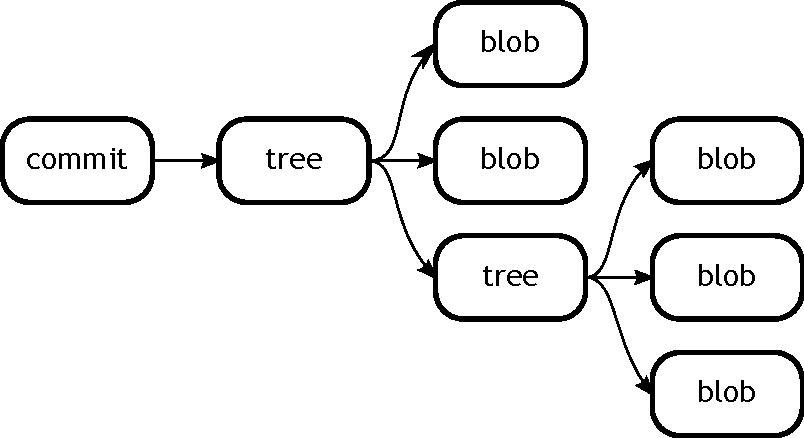
\includegraphics[width=9cm]{images/f-af2-d1.pdf}
\caption{Overview of objects in a repository}
\end{figure}

So now we know what a basic repository shuld look like, let us go through each stage of our committing in \textbf{Week 2} and see how it is built up at each stage.  Below is a consolidated list of all the objects in the repository.  

\begin{Verbatim}[frame=leftline,framerule=1mm,fontsize=\relsize{-3}]
./01/27bd2d49eea0820868fb2773461c3c0c7d874d		tree
./09/5b9cda52807c9c11781ec0a4aee927787b61f1		blob
./34/a5dff148e70c12310cda0800d6bcaf82530bdc		tree
./3a/d4cc3fe5a61c5563cb1b2ff3680d7e95be0fce		blob
./3f/fa7ab6dafef2bc38a70a39c53604c333ed4d7a		tree
./5d/2786685c15939fd93c66cd00dfdea4bd29da12		blob
./6c/a160c7226731bf80973fc5bc81f6b9beda7795		commit
./88/206926cb60aed53d21ede69f9ca5b7c69cb983		commit
./8d/664b74cce3a1f24d498d2d2bcc36e9915b5a65		tree
./96/551f45496232c0ec6b389731d55fa3d7e1c8fd		tree
./c9/887f89f1eed98d6b69124527a63f1149a7f927		blob
./e6/9de29bb2d1d6434b8b29ae775ad8c2e48c5391		blob
./e8/6ddea25341a75275d316d8ca545aa7c73e97b3		commit
./fa/65f06cc62291bb0cd47aef9e05953d6655fc8e		commit
\end{Verbatim}

